%-------------------------
% Resume in Latex
% Author : Aras Gungore
% License : MIT
%------------------------

\documentclass[a4paper,11pt]{article}

\usepackage{latexsym}
\usepackage[empty]{fullpage}
\usepackage{titlesec}
\usepackage{marvosym}
\usepackage[usenames,dvipsnames]{color}
\definecolor{cvlink}{rgb}{0.09,0.23,0.37}
\usepackage{verbatim}
\usepackage{enumitem}
\usepackage[colorlinks=true, linkcolor=cvlink, urlcolor=cvlink, citecolor=cvlink]{hyperref}
\hypersetup{
  pdftitle={Xiuyin Li - CV},
  pdfauthor={Xiuyin Li},
  pdfsubject={Research assistant application},
  pdfkeywords={reliable LLM agents, long-horizon interaction, agent systems, tool use, memory, RAG, empirical evaluation, failure analysis, uncertainty quantification, calibration, adaptation and transfer, controlled environments, interaction data}
}
\usepackage{fancyhdr}
\usepackage[english]{babel}
\usepackage[UTF8]{ctex}
\usepackage{tabularx}
\usepackage{hyphenat}
\usepackage{graphicx}
\graphicspath{{../assets/}{assets/}}
\usepackage{xparse}

%---------- FONT OPTIONS ----------
% sans-serif
% \usepackage[sfdefault]{FiraSans}
% \usepackage[sfdefault]{roboto}
% \usepackage[sfdefault]{noto-sans}
% \usepackage[default]{sourcesanspro}

% serif
% \usepackage{CormorantGaramond}
% \usepackage{charter}


\pagestyle{fancy}
\fancyhf{} % clear all header and footer fields
\fancyfoot{}
\renewcommand{\headrulewidth}{0pt}
\renewcommand{\footrulewidth}{0pt}
\setlength{\footskip}{4.08003pt}

% Adjust margins
\addtolength{\oddsidemargin}{-0.5in}
\addtolength{\evensidemargin}{-0.5in}
\addtolength{\textwidth}{1in}
\addtolength{\topmargin}{-.5in}
\addtolength{\textheight}{1.3in}

\urlstyle{same}

\raggedbottom
\raggedright
\sloppy
\setlength{\tabcolsep}{0in}

% Suppress font shape warnings.
\makeatletter
\def\font@warning#1{}
\def\@font@warning#1#2{}
\makeatother

% Sections formatting
\titleformat{\section}{
  \vspace{-4pt}\scshape\raggedright\large
}{}{0em}{}[\color{black}\titlerule \vspace{-10pt}]

%-------------------------
% Custom commands

\newcommand{\resumeItem}[1]{
  \item{\small
    {#1 \vspace{-4pt}}
  }
}


\newcommand{\resumeSubheading}[4]{
  \vspace{-2pt}\item
    \begin{tabular*}{0.97\linewidth}[t]{l@{\extracolsep{\fill}}r}
      \textbf{#1} & #2 \\
      \textit{\small#3} & \textit{\small #4} \\
    \end{tabular*}\vspace{-7pt}
}


\newcommand{\resumeSubSubheading}[2]{
    \vspace{-2pt}\item
    \begin{tabular*}{0.97\linewidth}{l@{\extracolsep{\fill}}r}
      \textit{\small#1} & \textit{\small #2} \\
    \end{tabular*}\vspace{-7pt}
}


\newcommand{\resumeEducationHeading}[9]{
  \vspace{-2pt}\item
    \begin{tabular*}{0.97\linewidth}[t]{l@{\extracolsep{\fill}}r}
      \textbf{#1} & #2 \\
      \small#3 & \textit{\small #4} \\
      \qquad \kaishu \small#5 \\
      \small#6 & \textit{\small #7} \\
      \qquad \kaishu \small#8 \\
    \end{tabular*}\vspace{#9}
}

\NewDocumentCommand{\resumeMultipleEducationHeading}{ O{-5pt} m }{%
  \vspace{-2pt}\item
  \begin{tabular*}{0.97\linewidth}[t]{@{}l@{\extracolsep{\fill}}l@{\extracolsep{\fill}}c@{\extracolsep{\fill}}r@{}}
    #2
  \end{tabular*}\vspace{#1}
}

\newcommand{\resumeProjectHeading}[2]{
    \vspace{-3pt}\item
    \begin{tabular*}{0.97\linewidth}{l@{\extracolsep{\fill}}r}
      \small#1 & #2 \\
    \end{tabular*}\vspace{-8pt}
}


\newcommand{\resumeOrganizationHeading}[4]{
  \vspace{-2pt}\item
    \begin{tabular*}{0.97\linewidth}[t]{l@{\extracolsep{\fill}}r}
      \textbf{#1} & \textit{\small #2} \\
      \textit{\small#3}
    \end{tabular*}\vspace{-7pt}
}

\newcommand{\resumeSubItem}[1]{\resumeItem{#1}\vspace{-4pt}}

\renewcommand\labelitemii{$\vcenter{\hbox{\tiny$\bullet$}}$}

\newcommand{\resumeSubHeadingListStart}{\begin{itemize}[leftmargin=0.15in, label={}]}
\newcommand{\resumeSubHeadingListEnd}{\end{itemize}\vspace{-15pt}}
% Research and project sections end with nested bullet lists, which need a
% little more space before the next section rule than tabular/list-only blocks.
\newcommand{\resumeDetailedSectionListEnd}{\end{itemize}\vspace{-10pt}}

\newcommand{\resumeItemListStart}{\begin{itemize}}
\newcommand{\resumeItemListEnd}{\end{itemize}\vspace{-10pt}}

%-------------------------------------------
%%%%%%  RESUME STARTS HERE  %%%%%%%%%%%%%%%%%%%%%%%%%%%%


\begin{document}

%---------- HEADING ----------
\vspace*{-1.0cm}
\begin{minipage}[c]{0.84\textwidth}
  \begin{raggedright}
    \textbf{\Huge Xiuyin Li}
    \hfill{\scriptsize\textcolor{Gray}{Last updated: \today}}
    \\
    \scriptsize
    \href{mailto:xiuyinli26@gmail.com}{xiuyinli26@gmail.com}
    \textbar{} \href{https://lixiuyin.github.io/}{lixiuyin.github.io}
    \textbar{} \href{https://github.com/lixiuyin}{github.com/lixiuyin}
    \textbar{} \href{https://www.linkedin.com/in/xiuyin-li/}{LinkedIn: xiuyin-li}
    \\
   \small Research assistant roles --- immediate availability; one-year minimum
   \textbar{} IELTS: 7.0 (W: 7.0, S: 6.5)
    \\
    \footnotesize Reliable LLM agents: systems, empirical evaluation, and failure analysis for long-horizon interaction
 \end{raggedright}
\end{minipage}
\hfill
\begin{minipage}[c]{0.12\textwidth}
  \raggedleft
  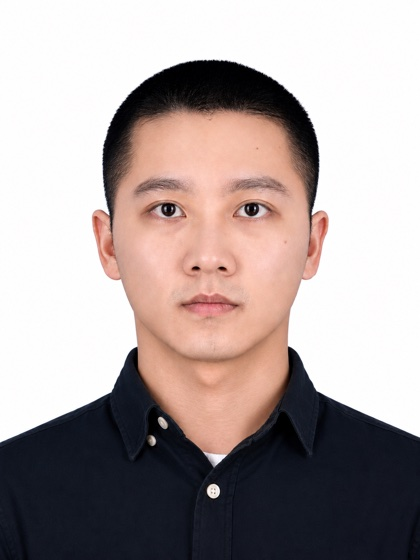
\includegraphics[width=\linewidth]{photo}
\end{minipage}

%----------- EDUCATION -----------
\vspace*{-0.6cm}
\section{Education}
\resumeSubHeadingListStart

  \vspace{-2pt}\item
  \begin{tabularx}{0.97\linewidth}[t]{@{}l@{\hspace{0.8em}}X@{\hspace{0.8em}}c@{\hspace{0.8em}}r@{}}
    \textbf{\href{https://www.hku.hk/about/uid/introduction.html}{The University of Hong Kong}} & {\small Master of Data Science} & \textit{\textbf{3.51/4.30}} & \textit{Sep 2025 -- Jul 2027 (expected)} \\
    \multicolumn{4}{@{}p{0.97\linewidth}@{}}{\small Deep Learning (A+), NLP and Text Analytics (A+), Data Mining (A-), Statistical Inference (A-), Advanced Statistical Modelling (A-), Programming for Data Science (A)}  \\[1pt]
    \multicolumn{4}{@{}p{0.97\linewidth}@{}}{\small Coursework completed; practicum remaining; degree requirements expected in December 2026.}  \\[1pt]
    \textbf{\href{https://www.en.sdu.edu.cn/info/1142/4095.htm}{Shandong University}} & {\small B.S. in Statistics} & \textit{\textbf{86.52/100}} & \textit{Sep 2021 -- Jun 2025} \\
    \multicolumn{4}{@{}p{0.97\linewidth}@{}}{\small Machine Learning (95), Statistical Computation (99), Bayesian Statistics (96), \mbox{Mathematical Statistics (92)}, \mbox{Multivariate Analysis (91)}, Python Programming (95), Database Technologies (99), Mathematical Modeling (90)}  \\[1pt]
    \multicolumn{2}{@{}l@{\hspace{0.8em}}}{\small Minor in Computer Science and Technology} & \textit{\textbf{88.86/100}} & \textit{Sep 2022 -- Jun 2025} \\
    \multicolumn{4}{@{}p{0.97\linewidth}@{}}{\small Data Structures (87), Operating Systems (91), Software Engineering (92), Object-Oriented Technology (90)} \\[1pt]
  \end{tabularx}\vspace{-5pt}

  \resumeSubHeadingListEnd

%----------- RESEARCH -----------
\vspace*{-0.12cm}
\section{Research Experience}
\resumeSubHeadingListStart

\resumeProjectHeading
  {\textbf{\href{https://github.com/lixiuyin/em-mcem-treg-mixed-models}{B.S. Thesis: EM and MCEM for Parameter Estimation in Regression Models}}}
  {\textit{May 2025}}
  \resumeItemListStart
    \resumeItem{Derived and implemented EM/MCEM in R for Student's \textit{t} regression and linear mixed models, including ECME and REML updates; validated in 200- and 500-replication simulations and against standard R packages.}
    \resumeItem{Reworked computations to avoid dense matrices for 8,000 UTKFace embeddings and 59,699 CIFAR-10H trials; the \textit{t} model outperformed a Gaussian baseline in-sample, while the mixed model matched \texttt{lme4}.}
  \resumeItemListEnd

\resumeProjectHeading
  {\textbf{Synthetic Control Methods for Causal Inference}}
  {\textit{Research Collaboration \textperiodcentered{} Jul--Aug 2024}}
  \resumeItemListStart
    \resumeItem{Explored synthetic-control applications and extensions with \href{https://scholar.google.com/citations?user=oBPd6C0AAAAJ}{Yunhao Wang} and three other undergraduate students through reading and reproduction of R studies spanning design and treatment-effect estimation.}
  \resumeItemListEnd
\resumeDetailedSectionListEnd

%----------- PROJECTS -----------
\vspace*{-0.12cm}
\section{Selected Projects}
\resumeSubHeadingListStart

\resumeProjectHeading
  {\textbf{\href{https://github.com/lixiuyin/meeting-agent}{Meeting Agent --- Multimodal Hybrid RAG with Long-Term Memory}}}
  {\emph{Project Lead \textperiodcentered{} Apr 2026}}
  \resumeItemListStart
    \resumeItem{Designed and implemented a hierarchical hybrid RAG over meeting transcripts, parsed text, OCR, and image captions, combining Chroma retrieval with SQLite FTS5/BM25, RRF, and semantic reranking.}
    \resumeItem{Evaluated retrieval with Recall, MRR, and nDCG; used LLM-as-judge scores for faithfulness, relevance, and context precision; tested memory persistence, ingestion, streaming, and failure recovery.}
    \resumeItem{Added cross-session memory with LLM-extracted facts, semantic retrieval, TTL/importance decay, alias-aware entities, and episodic summaries for persistent recall across meetings.}
  \resumeItemListEnd

\resumeProjectHeading
  {\textbf{\href{https://github.com/lixiuyin/web-agent}{WebAgent --- Browser Agent \& Evaluation Harness}}}
  {\emph{Project Lead \textperiodcentered{} Nov 2025--Present}}
  \resumeItemListStart
    \resumeItem{Built a model-agnostic Chromium agent with screenshot-and-DOM grounding, policy-gated typed tools, atomic checkpoint recovery, and caption-grounded PDF analysis across hosted APIs and local vLLM.}
    \resumeItem{Developed versioned traces and a 36-task harness across public web, sandbox, and forced resume, with independent judging and confidence calibration; on one frozen date, both models passed 35/36.}
\resumeItemListEnd

\resumeProjectHeading
  {\textbf{\href{https://github.com/lixiuyin/zero-shot-cnn-textual-description-reproduction}{Zero-Shot CNNs from Textual Descriptions -- Reprod. \& Ext.}}}
  {\emph{Project Lead \textperiodcentered{} Mar 2026}}
  \resumeItemListStart
    \resumeItem{Implemented the core \href{https://arxiv.org/pdf/1506.00511}{Ba~et~al. (ICCV 2015)} zero-shot CNN predictors in PyTorch from scratch, generating class-specific FC/conv weights from text for unseen classes under a paper-aligned seen/unseen protocol.}
    \resumeItem{Ran paper-aligned CUB/Flowers evaluation plus 13 extensions (3 losses, 4 SBERT/CLIP variants, 6 backbones); with joint/VGG-19/BCE fixed, multi-granularity CLIP achieved unseen-class ROC-AUC 0.680$\to$0.886.}
  \resumeItemListEnd
\resumeDetailedSectionListEnd

%----------- TEACHING -----------
\vspace*{-0.12cm}
\section{Teaching}
\vspace{1pt}
  \resumeSubHeadingListStart
    \small{\item{
        \textbf{Teaching Assistant, Shandong University} --- Mathematical Analysis I \& II, PDE \hfill \textit{Sep 2024 -- Jun 2025} \\ \vspace{3pt}
        Graded homework and answered questions; translated PDE slides and assisted with calculus-textbook LaTeX.
    }}
  \resumeSubHeadingListEnd

%----------- SKILLS -----------
\vspace*{-0.12cm}
\section{Skills}
\vspace{1pt}
  \resumeSubHeadingListStart
    \small{
      \item{
        \textbf{Machine Learning \& AI:}
        PyTorch, scikit-learn; Hugging Face Transformers, PEFT/LoRA, vLLM \\[2pt]
        \textbf{Agents \& Evaluation:}
        LangChain, ReAct, MCP, Playwright/CDP, Pydantic, agent orchestration, offline evaluation \\[2pt]
        \textbf{Statistics \& Modeling:}
        Python, R, SQL; NumPy, pandas, SciPy; mixed-effects modeling \\[2pt]
        \textbf{Software \& Reproducibility:}
        Git, Linux (CLI), Docker, pytest, CI/CD, conda/uv, \LaTeX; C++, Java
      }}
  \resumeSubHeadingListEnd


%----------- EXPERIENCE -----------

% \section{Work Experience}
%   \vspace{3pt}
%   \resumeSubHeadingListStart
%
%     \resumeSubheading
%       {Avikon}{Istanbul, Turkey}
%       {Software Engineer}{December 2023 \textbf{--} Present, Full-time}
%         \resumeItemListStart
%             \resumeItem{Designed a Qt-based chat application using TCP for real-time communication in a client-server architecture, demonstrating expertise in socket programming, data serialization, and message routing.}
%             \resumeItem{Designed message types in IDL and built a data-centric publish-subscribe architecture for an OpenDDS radar command-and-control interface using the Flyweight design pattern. Used QoS policies to support volatile and persistent data transfer across topics.}
%             \resumeItem{Implemented a fully asynchronous AMQP-based C++ client with a layered architecture for RabbitMQ, ensuring seamless message handling across topics.}
%             \resumeItem{Developed a cross-platform asynchronous program to improve drone detection in GIS applications. Benchmarked point-in-polygon algorithms using a GeoJSON polygon database fetched concurrently from MongoDB.}
%         \resumeItemListEnd
%
%   \resumeSubHeadingListEnd

%----------- RELEVANT COURSEWORK -----------

% \section{Relevant Coursework}
%   \vspace{2pt}
%   \resumeSubHeadingListStart
%     \small{\item{
%         \textbf{Major Courses:}{Mathematical Analysis, Advanced Algebra, Ordinary Differential Equations, Probability Theory, Mathematical Statistics, Real Analysis, Functional Analysis, Applied Regression Analysis, Operations Research, Bayesian Statistics, Fundamentals of Stochastic Processes, Multivariate Statistical Analysis, Time Series Analysis, Java Programming, Python Programming, Statistical Computing, Machine Learning, Data Structures} \\ \vspace{3pt}
%
%         \textbf{Minor Courses:}{Discrete Mathematics, Object-Oriented Programming, Data Structures, Database Systems, Java Programming, Computer Organization, Software Engineering, Machine Learning, Computer Networks, Web Technology, Operating Systems}
%     }}
%   \resumeSubHeadingListEnd



%----------- CERTIFICATES -----------

% \section{Certificates}
  % \resumeSubHeadingListStart

    % \resumeOrganizationHeading
      % {Procter \& Gamble VIA Certificate Program}{Feb 2022}{Project Management and Personal Productivity}

  % \resumeSubHeadingListEnd



%----------- ORGANIZATIONS -----------

% \section{Organizations}
  % \resumeSubHeadingListStart

    % \resumeOrganizationHeading
      % {Institute of Electrical and Electronics Engineers (IEEE)}{Feb 2022 -- Present}{Student Member}

  % \resumeSubHeadingListEnd



%----------- HOBBIES -----------

% \section{Hobbies}
  % \resumeSubHeadingListStart
    % \small{\item{Basketball, Swimming, Fitness, Eight-ball, Horology}}
  % \resumeSubHeadingListEnd



%----------- REFERENCES -----------

% \section{References}
  % \vspace{2pt}
  % \resumeSubHeadingListStart
    % \item{References available upon request.}
  % \resumeSubHeadingListEnd



%----------- AWARDS & ACHIEVEMENTS -----------
% \vspace*{-0.12cm}
% \section{Selected Awards}
%   \resumeSubHeadingListStart
%     \small{\item{
%         \textbf{Mathematical Contest in Modeling} --- Honorable Mention \hfill \textit{Feb 2024} \\ \vspace{3pt}
%         \textbf{China Undergraduate Mathematical Contest in Modeling} --- First Prize (Shandong) \hfill \textit{Sep 2023} \\ \vspace{3pt}
%     }}
%   \resumeSubHeadingListEnd

%-------------------------------------------
\end{document}
